\documentclass[10pt,letterpaper]{article}
\usepackage[margin=0.75in]{geometry}
\usepackage{listings}
\usepackage{color}
\usepackage{longtable}
\usepackage{tabu}
\usepackage{pgfplots}

\definecolor{dkgreen}{rgb}{0,0.6,0}
\definecolor{gray}{rgb}{0.5,0.5,0.5}
\definecolor{mauve}{rgb}{0.58,0,0.82}

\lstset{frame=tb,
  language=C,
  columns=flexible,
  numberstyle=\tiny\color{gray},
  keywordstyle=\color{blue},
  commentstyle=\color{dkgreen},
  stringstyle=\color{mauve},
  breaklines=true,
  breakatwhitespace=true,
  tabsize=4
}

\begin{document}
\begin{titlepage}
  \title{CS 331 - Spring 2016 - Implementation 1}
  \author{Cody Malick - Andrew Tolvstad\\
  \texttt{malickc@oregonstate.edu}, \texttt{tolvstaa@oregonstate.edu}}
  \date{\today}
  \maketitle
  \vspace*{2cm}

\end{titlepage}

\section{Implementation Assignment 1}
	\subsection{Methodology}
	\subsubsection{Breadth-First Search}
Getting this algorithm working was quite a bit of trial and error, as fully
expanding all possible nodes until a solution is found is memory intensive.
We implemented this algorithm using queue for the general data structure, we
used a set data structure containing tuples representing individual states
visited, and a trace function "ascend()" to return the path the algorithm takes
to find the solution.


	\subsubsection{Depth-First Search}
Depth-first was much faster than BFS. The only difference between this and BFS
was that we used a double-ended queue for our data structure.

	\subsubsection{Iterative Deepening Depth-First Search}
This is identical to DFS, with the added element of a maximum depth variable.
Through some experimentation, we found that a solution could be found at X depth.
We tried many different depths, such as the depth found with the result of running
straight DFS which was X. For each of the test files, here were the depths we
used to find solutions for the corresponding test cases:
\begin{enumerate}
  \item
  \item
  \item
\end{enumerate}

	\subsubsection{A-Star Search}
Stuff, explanation of heuristic

  \subsection{Results}
  Here are the results of our implmentations:


  \begin{center}
      \begin{tabular}{ | l | p{2cm} | p{2cm} | p{2cm} |}
      \hline
      & Test Case 1 & Test Case 2 & Test Case 3 \\ \hline
      BFS & Path:29  Nodes:2971 & Path:52  Nodes:12305  & Path:  Nodes: \\ \hline
      DFS & Path:40  Nodes:58 & Path:82  Nodes:165 & Path:5256  Nodes:11040 \\ \hline
      IDDFS & Path:  Nodes: & Path:  Nodes: & Path:  Nodes: \\ \hline
      A-Star & Path:  Nodes: & Path:  Nodes: & Path:  Nodes: \\ \hline
      \end{tabular}
  \end{center}


	Here is a graph illustrating the results of our executions:
  \subsubsection{graph}
    \begin{center}
    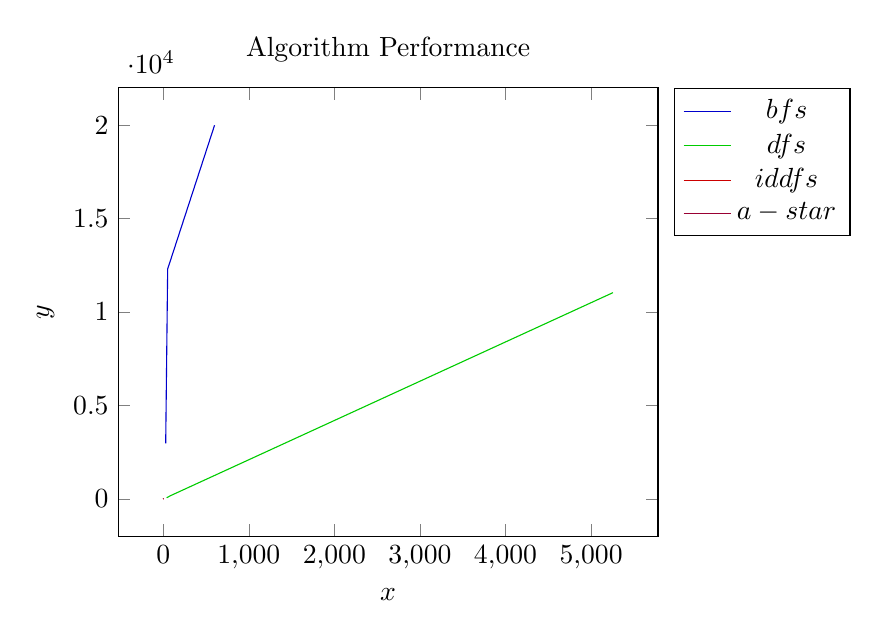
\begin{tikzpicture}
      \begin{axis}[
        title=Algorithm Performance,
        legend pos=outer north east,
        xlabel=$x$,
        ylabel={$y$}
        ]
        \addplot[blue!80!black]
          coordinates
          {(29,2971)(52,12305)(600, 20000)};
        \addplot[green!80!black]
          coordinates
          {(40,58)(82,165)(5256,11040)};
        \addplot[red!80!black]
          coordinates
          {(1,3)(2,4)(2,5)(3,6)(4,7)};
        \addplot[purple!80!black]
          coordinates
          {(1,4)(2,5)(2,6)(3,7)(4,8)};
          \legend{{$bfs$},{$dfs$},{$iddfs$},{$a-star$}}
        \end{axis}
    \end{tikzpicture}
  \end{center}

  \subsection{Discussion}
  Overall the results for breadth-first were expected. BFS is very inefficient.
  After implementing the signature vector, our implmentation had a much easier
  time finding the solution on smaller data sets, eliminating repeated states.

  This still only reduced the problem size slightly. We were still iterating
  over an enormous tree to find the solution.

  We had quite a time running this algorithm against test case three, containing
  eighty-eight missionaries and eighty cannibles. Before sorting out a few memory
  leaks (we implmented all our algorithms in C++), we were hitting thirty-plus
  gigabytes of RAM while BFS was trying to resolve the solution. Luckly, we were
  able to resolve the memory issue, and BFS on that size array eventually
  terminated.

  Depth-first was quite a different experience from BFS. We implemented it using
  a double-ended queue. Depth-first was able to resolve the solutions for all three test cases quickly
  and efficiently, contrary to what we believed would happen. We (Andy and Cody)
  thought it would be as slow or slightly faster, but it ended up being drastically
  better in performance and number of steps taken.

  Iterative Deepening Depth-First was a nice improvement over DFS, and much, much
  better than BFS. By implementing the hard limit on depth and only increasing that
  when we need to, we get the best solution across multiple branches quickly.



  \subsection{Conclusion}
  From these results, we can see that XXX search is the most efficient of these four.
\end{document}
